\documentclass[11pt]{article}

\title{ExploitFarm Project}
\usepackage{graphicx}
\usepackage[utf8]{inputenc}
\usepackage{hyperref}
\author{Domingo Dirutigliano}

\begin{document}

\begin{titlepage}
   \begin{center}
       \vspace*{1cm}

       \LARGE{\textbf{ExploitFarm Project}}

       \vspace{0.5cm}
        Analisi di progetto e documentazione
       
       \vspace{0.5cm}
       
       \begin{figure}[h]
    		\centering
    		
\includegraphics[width=0.2\textwidth]{logo.png}
		\end{figure}
       
       \vspace{0.5cm}

       \textbf{Domingo Dirutigliano}

       \vfill
            
       Politecnico di Bari\\
       Software Engineering
            
       \vspace{0.1cm}
   \end{center}
\end{titlepage}

\tableofcontents
\newpage

\section{Introduzione}
\subsection{Descrizione generale}
	"Exploitfarm" è un software completamente dedicato alle competizioni CTF Attack/Defence, che si occupa principalmente di gestire la fase di attacco e ti tutto quello che conseguentemente questa fase richiede per essere eseguita correttamente, al fine di semplificare e velocizzare gli attacchi.\\
	In generale Exploitfarm si occupa di attaccare in parallelo una serie di team (attacker) e di raccogliere ed inviare seguendo i criteri e limitazioni indicate per la competizione che si sta svolgendo le flag al gameserver (submitter).
\subsection{Obiettivi}
\begin{itemize}
    \item Setup e installazione facile, veloce, personalizzabile e facilmente automizzabile
    \item Gestione delle risorse per gli attacchi dinamica e reattiva
    \item Scrittura degli exploit e dei test su questi semplificata
    \item Interfaccia intuitiva con avvio e configurazione intuitiva e rapida
    \item Keep track of anything: accumula dati sugli attacchi e ne permette un'analisi veloce ed intuitiva
    \item Rende semplice la condivisione/collaborazione sugli attacchi e la loro esecuzione
    \item Leggero da eseguire su qualsiasi piattaforma
    \item Gestione distribuita degli attacchi
\end{itemize}
\subsection{Perchè lo sviluppo di un nuovo attacker/submitter?}
Gli attacker attualmente esistenti sono spesso incompleti, difficili da configurare e da completarne il setup, facilmente inclini ad errori che spesso comportano una perdita di tempo aggiuntiva, non hanno alcun tipo di gestione del carico supportato dalla macchina che esegue gli attacchi, non memorizza o espone alcun dato statistico sull'andamento degli attacchi ed infine non gestisce la condivisione degli exploit stessi.\\
Date le forti lacune presenti in software simili già esistenti, ho ritenuto opportuno la creazione di un'alternativa agli attacker attualmente esistenti.\\
\textbf{NOTA}: "ExploitFarm" è liberamente ispirato ad un altro attacker molto famoso chiamato \href{https://github.com/DestructiveVoice/DestructiveFarm}{DestructiveFarm}, ma ne condivide a livello di codice unicamente delle piccole porzioni del suo client "start\_xploit.py" a loro volta modificate ed adattate, in alcune parti riscritte e riprogettate completamente date le netti differenze di requisiti dei progetti.
\section{Specifiche}
\subsection{Composizione del progetto}
Il progetto è composto principalmente da un server centrale (nello specifico un web server) che coordinerà una serie di client sia frontend (web) che tramite una CLI. La parte di coordinamento, di submitting e gestione dei dati è affidata al server.
    \begin{figure}[h]
    	\centering
    	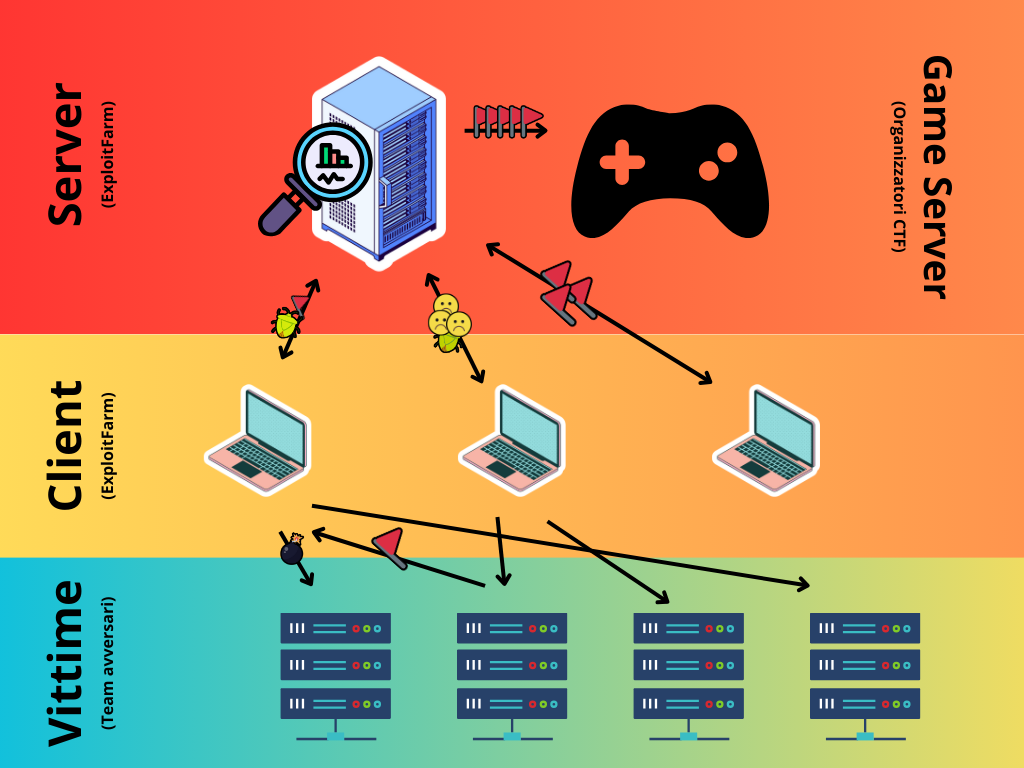
\includegraphics[width=1\textwidth]{general_layout.png}
	\end{figure}
\subsubsection{Backend}
Il backend sarà il core del progetto poiché conterrà tutta la logica per il coordinamento dei vari client che invieranno il risultato degli attacchi, dovrà gestire i dati ed elaborarli al fine di renderli facilmente fruibili dai client, inoltre conterrà la logica e si occuperà della gestione del submitting delle flag al gameserver seguendo i requisiti indicati in fase di setup.
\subsubsection{Frontend}
La visualizzazione avanzata dello stato di ExploitFarm è invece affidata alla parte frontend del webserver che dovrà permettere un facile accesso ai dati presenti sul server, offrendoli tramite strumenti di analisi come grafici che devono essere mirati sulle esigenze decisionali che possono emergere durante una competizione Attack Defence. Inoltre dovrà segnalare e rendere facilmente e tempestivamente nota la presenza di eventuali errori di qualsiasi tipo sull'intera infrastruttura permettendone un'intervento quanto più immediato da parte del team.
\subsubsection{CLI (xfarm)}
Infine un'ultima parte fondamentale in tutto il progetto è il client che deve essere eseguito preferibilmente su macchine diverse da quella che offre il server, che si occupa dell'esecuzione stessa degli attacchi, della creazione del progetto dell'attacco, del monitoraggio (parziale) dell'attacco stesso. Anche il client stesso dovrà avere un'interfaccia in questo caso TUI intuitiva e veloce da utilizzare che deve rendere immediato e facile l'avvio dell'attacco e l'inserimento dei dati richiesti per l'esecuzione dell'attacco stesso.
\subsection{Specifica dei requisiti}
\subsubsection{Setup}
Il setup di ExploitFarm dalla sua installazione alla conclusione della sua configurazione deve essere di facile ed intuitivo utilizzo e di semplice finalizzazione. Al fine di perseguire questo obiettivo[...]
\subsubsection{Gestione Exploit}
\subsubsection{Esecuzione Attacchi}
\subsubsection{Analisi statistiche e visualizzazione}
\subsubsection{Gestione di attacchi distribuiti}
\subsection{Specifiche Tecniche}
\subsubsection{Gestione funzionalità backend}
\subsubsection{Funzionalità frontend}
\subsubsection{Strutturazione del client (xfarm)}
\subsubsection{Autobilanciamento del carico sul client per l'esecuzione degli attacchi}
\subsubsection{Gestione e versioning degli exploit}
\subsubsection{Controllo distribuito degli attacchi condivisi}
\section{Modello di Business}
\section{Analisi SWOT}
\section{Sviluppi Futuri}
Server Multipli e Decentralizzati

\end{document}
